\subsubsection{Ausrichtung Drehturm}
\begin{figure}[h!]
	\centering
	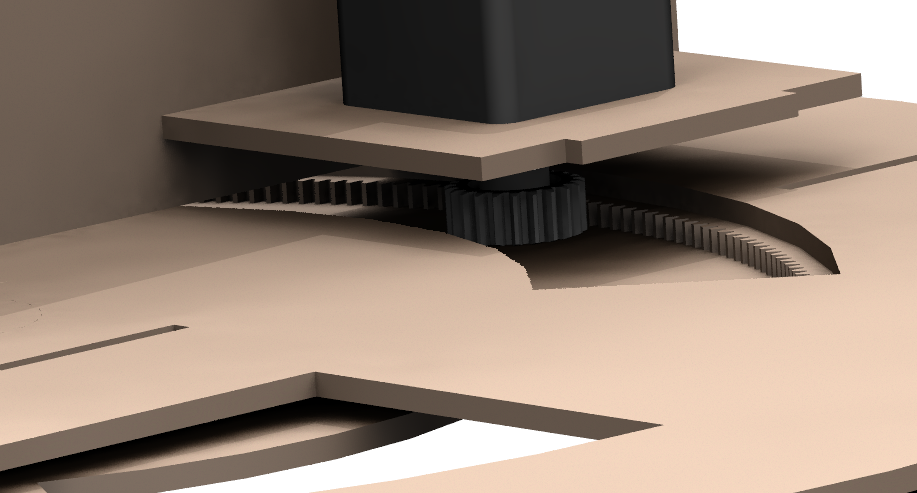
\includegraphics[width=\linewidth]{../../fig/Drehmechanismus}
	\caption{Drehmechanismus}
	\label{fig:Drehmechanismus}
\end{figure}
\paragraph{Komponentenbeschrieb}
Die horizontale Ausrichtung der Maschine in Richtung des Korbes, wird mittels einem Schrittmotor ermöglicht. An der Antriebswelle des Motors ist ein Kunststoff-Zahnrad angebracht, welches in ein eigens konstruiertes Hohlrad-Segment eingreift und somit durch Rotation eine Drehung des Drehturmes bewirkt. Dieses Segment ist auf der Grundplatte befestigt, welche fix auf dem Tisch liegt. Die zwei Platten, sowie das Hohlrad-Segment wurden mit NX konstruiert und mit einer Laserschneidmaschine aus MDF gefertigt.

\paragraph{Entwicklungsprozess}
Gemäss Aufgabenstellung sollen sich nach Abschluss des Wurfvorganges fünf Bälle im Korb befinden. Da die Position des Korbes nicht fix vorgegeben ist, können die Bälle nicht einfach nach vorne befördert werden. Um die Wurfvorrichtung ausrichten zu können, musste daher ein weiterer Aktor her. Grundsätzlich standen zwei Lösungskonzepte zur Auswahl. Ein seitliches Verschieben der kompletten Maschine, oder eine stationäre Variante mit einem Drehturm. Da eine seitliche Verschiebung in vielerlei Hinsicht schwieriger auszuführen wäre, entschied man sich für die Eigenrotation. Aus Montage- und Kostengründen verzichtete man bei der Lagerung zwischen den beiden Grundplatten auf ein genormtes Lager, obwohl dieses in der Planung vom PREN 1 vorgesehen wurde. Dieses Lösungskonzept verursacht jedoch eine höhere Reibung, weshalb der Schrittmotor eine grössere Leistung aufweisen muss. Dies stellt für den gewählten Motor allerdings kein Problem dar.